\documentclass[UTF8]{csoarticle}


\newtheorem{theorem}{定理}
\newtheorem{lemma}{引理}
\renewcommand{\proofname}{证明}
% 如果为英文文章,可以使用下面的定义(去除行首的注释符号%)代替上述中文定义
% \newtheorem{theorem}{Theorem}
% \newtheorem{lemma}{Lemma}

\begin{document}

%----------------------------------------------------------
% 1. 文章标头信息
%----------------------------------------------------------

\titleCHN{基于局部特征的图像重建算法}
\titleENG{Image Reconstruction Based on Local Features}
\authorCHN{王继哲\affil{1},李学明\affil{2}}
\authorENG{WANG Ji-Zhe\affil{1}, LI Xue-Ming\affil{2}}
\affiliationCHN{
    \affil{1} 北京邮电大学信息与通信工程学院,北京 100876 \\
    \affil{2} 北京邮电大学信息与通信工程学院,北京 100876
}
\affiliationENG{
    \affil{1} School of Information and Communication Engineering, Beijing University of Posts and Telecommunications, Beijing 100876 \\
    \affil{2} School of Information and Communication Engineering, Beijing University of Posts and Telecommunications, Beijing 100876
}

\abstractCHN{基于局部特征的图像重建算法是利用原始图像的局部特征信息,以大图像集为数据源,进行较为精确的图像重建工作,使重建后的图像与原始图像相似,并且图像质量达到人眼主观效果较好的程度。本文首先对目前图像重建算法加以概述,综合介绍重建系统中的局部特征、视觉词组、相似图像搜索、特征匹配、特征配准、匹配特征块筛选、图像融合等多种计算机视觉相关技术。之后将该系统引入大语料集的应用场景下,对上述几个环节进行完善,主要包括在在匹配块筛选法中提出阈值自适应的验证准则,为匹配块的筛选提供更有力的依据,显著提升了拼接结果。同时在相似图像搜索中使用分块查询技术,保证了搜索结果的多样性;}

\abstractENG{abstract text}
\keywordCHN{中文关键词要能反映文章的基本观点,避免广义词。第一个关键词为该文内容所属二级学科名称}
\keywordENG{list of keywords}
\cateidCHN{请查阅《中国图书馆分类法》}

\authorIntroduction{王继哲(1989-),男,硕士研究生,主要研究方向:多媒体通信,图像处理。通信作者:李学明(1969-),男,教授,主要研究方向:多媒体通信,图像处理。}
\fund{***基金(00000000),***基金(00000000)}

\maketitle


%----------------------------------------------------------
% 2. 正文内容
%----------------------------------------------------------

\section{引言}

随着移动终端计算能力的提升,终端应用迎来蓬勃发展,图片类应用日益普及,每天有数以万计的高分辨率图像由移动终端上传到服务器上,给通信网络带宽造成了巨大的压力。
另一方面我们观察到随着存储设备容量变大、芯片计算能力的提升,互联网用户的不断增多,大数据时代来临。图像数据数以亿计,服务器计算能力极大提升。从信息的角度来说,我们拍摄的每一幅图像中所包含的部分或全部内容都可以在互联网上其它图像中找到。

在2013年有学者[文献6]提出一种全新的压缩方式——基于云的图像编码。其核心思想是在客户端提取并编码发送少量的图像特征数据,并不传输图像数据本身,而在服务器端解码后利用特征数据在服务器的大图像数据集上匹配相似的图像,利用相似图像进行图像的重建。这种架构所运用的核心技术手段便是基于局部特征的图像重建算法。系统的核心思想是通过对原始图像的特征提取与重建,利用计算资源减少带宽损耗,从一个全新的维度进行数据压缩,为多媒体应用开启了一扇大门。

图像重建任务的核心是通过局部特征找到与原始图像相似的图像单元以及可靠的图像间对应点集合,进而自动地建立图像之间点与点或区域与区域之间的可靠对应关系,根据对应关系采用一定的算法拼接图像单元。基于局部特征对图像进行重建的技术能够让我们在发送端只传输少量的特征数据,而接收端服务器利用大数据集进行高分辨率图像的还原。



\section{重建算法系统概述}
%介绍Cloud Coding 系统的概要
文献\cite{Cloud}创新性的提出了基于云的图像编码方式,核心思想是以客户端进行特征提取,在服务器端利用局部特征在大规模图像集上找到相匹配的图像块,利用计算机视觉相关算法将图像块拼合成一幅完整图像,达到图像重建的目的。重建的流程如图\ref{fig:flow}所示:

\begin{figure}
\centering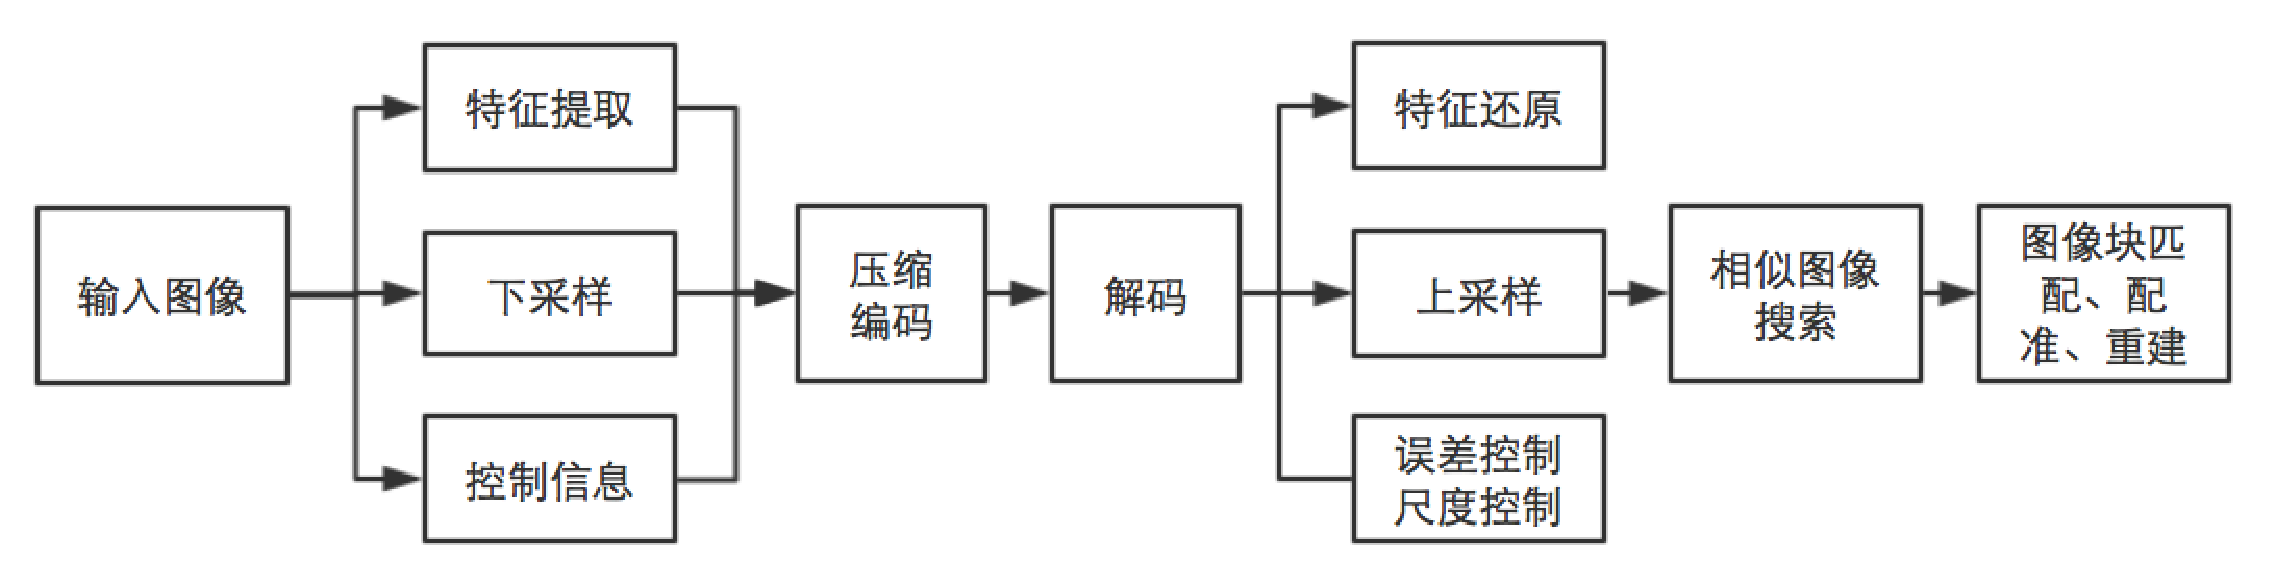
\includegraphics[width=15cm]{flowchart}
\caption{重建算法流程图}
\label{fig:flow}
\end{figure}

本文在上述的大框架下综合使用多种信息检索与图像处理技术,使用了上述系统中相同的数据编解码方式,而对对其中的相似图像检索、图像块筛选等核心算法进行了改进与完善,使之更加能够适用于大规模图像集上的图像重建任务,重建速度得到提升,重建结果得到了进一步的优化。

\section{基于局部特征的图像重建算法}
在本文的应用场景下,图像重建的部分流程可以看成是多幅图像的全景图拼接问题。与文献\cite{Brown:2006ir}中的流程类似,主要包含以下几个环节:(1)使用具有不变性的特征来描述图像;(2)自动的找到图像之间的空间位置关系,进行图像配准;(3)图像融合,消除不同图像之间的光照差别,去除边缘噪声。与全景图拼接不同的是,本文的图像重建系统以图像块(Patch)和上采样图像为输入,如何解决图像块大小不一空间位置以及像素值准确度低的问题,如何充分利用上采样图像信息优化图像融合是本文尝试解决的问题,现分别介绍如下。

\subsection{图像的局部特征}
图像的局部特征是计算机视觉领域一个基本问题,它能够反映图像某一局部的特性,对寻找图像对应的局部单元以及特征描述中有着重要作用。描述的核心问题是不变性和可区分性。

在多种局部特征中,本文选择使用Lowe提出的尺度不变特征变换(Scale Invariant Feature Transform,以下简称SIFT)。SIFT算子是图像局部特征研究领域的一项重大突破。SIFT算子具有很强的可区分性,同时对尺度、旋转以及一定视角和光照变化等图像变化都具有不变性。

\subsubsection{尺度空间理论}
尺度空间是模拟图像数据的多尺度特征:尺度空间中图像的模糊程度逐渐变大,能够模拟人在距离目标由近到远时目标在视网膜上的成像过程。我们可以把两幅图像想象成是连续的,分别以它们作为底面作四棱锥,就像金字塔,那么每一个截面与原图像相似,金字塔的两层中包含无穷个截面,在实际应用只能选择离散诘责,构造有限个层。

\subsubsection{SIFT检测子与描述子}
SIFT算法有两个主要环节,一个是检测“感兴趣”的关键点,另一个是描述这个“关键点”。SIFT关键点是精心选择的一组在高斯差分尺度空间上的极值点,该关键点表示成\((x_f,y_f,s_f,\theta)\),包含三个关键信息,分别是(1)亚像素精度的(x,y)位置信息;(2)尺度大小,反映关键点局部的大小,同时决定了特征的覆盖范围,对后文局部块的提取起到至关重要的作用;(3)所在高斯尺度空间上的主方向,该主方向是有一个高斯窗口函数计算得来,反映的是关键点所在局部的方向信息。

SIFT描述子反映关键点局部的信息,是高斯尺度空间上某一局部和方向上的梯度信息,以直方图的形式对信息做统计,最终每一个描述子是一个128的特征。

\subsection{特征匹配}
当我们通过相似图像搜索获得与原图近似的图像后,需要精确的找到原始图像与候选拼接图像相匹配的特征点,其匹配策略为:
\begin{equation}
  M(S_1,S_2) = 
\begin{cases} 
\text{true}, & \mbox{if } S_2 = S_{min},\frac{\text{Dis}(S,S_{min})}{\text{Dis}(S,\tilde{S}_{min})} > C \\
\text{false}, & \mbox{otherwise}
\end{cases}
\end{equation}
其中\(\text{Dis}(\cdot,\cdot)\)表示的是两个特征描述子之间的相似性度量,比如可以用欧氏距离表示,距离越大,相似性越小。\(S_{min}\)和\(\tilde{S}_{min}\)分别表示的是与S距离最近和第二近的特征。而C是一个阈值常数,通常取1.5。当原图特征点比较多时,为了提升匹配速度和匹配精度,可以适当提高该常数。

匹配通常采用k-d树\cite{李航2012统计学习方法}技术进行最近邻搜索。对于n个实例的k维数据来说,建立kd-tree的时间复杂度为O(k*n*logn)。时间复杂度比暴力法要降低很多。

\subsection{图像配准}
匹配完成后,原始图像的SIFT特征\(S\)匹配到了候选图像中的特征\(\tilde{S}\),通过匹配的特征对我们可以得到两个对应的图像块,原图图像块\(P_S\)和候选图像块\(P_{\tilde{S}}\),图像块是根据SIFT特征以及对应的图像得到的。本文选取的是正方形图像块,其中尺度决定了图像块的大小。

当一个图像块中的多个SIFT特征匹配之后,我们找到了多个匹配的图像块,这时每对图像块都是正方形构成,我们希望对候选图像块做进一步的投影变换,使之与原图像块更为精准的匹配,这一环节叫做图像配准。

根据文献\cite{Dai:2012vn},有两种配准方式,一种是直接写出变换矩阵,另一种是使用RANSAC方式多次迭代找到最准确的变换矩阵。RANSAC的方式将在后文介绍,我们先介绍根据一对匹配的SIFT算子直接写出两个图像块的变换矩阵。

结合一对匹配SIFT特征点\(\tilde{S}\)和\(S\)的位置、尺度和方向,我们可以得到两个图像块\(P_{\tilde{S}}\)和\(P_S\)的变换矩阵\(H_0\):

\begin{equation}
  H_0 = 
  \begin{bmatrix}
  \frac{\tilde{s}_f}{s_f} R & T
  \end{bmatrix}
\end{equation}
其中
\begin{equation}
  R = 
  \begin{bmatrix}
    \cos{(\tilde{\theta}-\theta)} & -\sin{(\tilde{\theta}-\theta)} \\
    \sin{(\tilde{\theta}-\theta)} & \cos{(\tilde{\theta}-\theta)} 
  \end{bmatrix}
\end{equation}

\begin{equation}
  T = 
  \begin{bmatrix}
    \tilde{x}_f - x_f \\
    \tilde{y}_f - y_f
  \end{bmatrix}
\end{equation}

计算出的\(H_0\)和\(H\)都可以作为块的旋转矩阵,在实际的系统中,我们会同时计算两个矩阵,比较他们的准确程度,挑选使用准确度高的变换矩阵,在实验中,因为我们采用上采样图像的均方误差做验证,而上采样图像本身的精度损失导致误差估计不准确,所以我们采用如下的策略:当匹配块内匹配特征点多时,我们更倾向于使用RANSAC算法计算得到的变换矩阵,反之我们更倾向于使用直接计算法。

\subsection{自适应图像块筛选法}
图像重建任务的最后一个步骤是图像融合,在此之前我们已经得到了每个原图像特征对应的候选图像块,图像块的方向、尺度、位置都有所不同,图像块之间可能存在交叠,部分图像块与原图存在较大误差,需要利用上采样图像计算配准后的图像块与原图像块的误差,根据设定好的阈值\(\epsilon\)移除误差较大的图像块。

在文献\cite{Dai:2012vn}中作者提到使用对上述配准后的图像块使用基于图的图像分割方案,对每一个分割连通域做均方误差校验,相当于图像块做进一步的细分,能够有效去除图像块中不匹配的部分。在实际测试中,由于我们在高分辨率图像重建场景下,导致图像分割与图像像素数量成正比,资源消耗过大,另一方面分割导致图像粒度过细,验证步骤的误差存在难以保证筛选结果的准确,因此我们在此省略了精细化分图像块的步骤,提出了一种自适应阈值的图像块筛选法。

原图像经过特征提取、过滤操作后,有几百个大尺度图像块,在分布密集区域,图像块有大量的重叠,并不需要对每一个候选图像块做最后的拼接。利用相似图像搜索得到候选图像,在候选图像中利用特征匹配找到原图像块匹配的候选图像块,虽然在SIFT描述子级别上两个候选图像块是匹配的,但无法保证像素级别上的一致。

在文献\cite{Dai:2012vn}中,使用上采样图像\(I_u\)来校验候选图像块是否正确。校验规则为是

\begin{equation}
  \text{Verify}(P_{\tilde{S}}) = 
\begin{cases} 
\text{true}, & \mbox{if MSE} (T(P_{\tilde{S}}),P_c \in I_u) < \epsilon \\
\text{false}, & \mbox{otherwise}
\end{cases}
\end{equation}

其中\(\text{MSE}(\cdot,\cdot)\)表示的是两个图像块的均方误差(Mean Square Error)。\(T(P_{\tilde{S}}\)表示对候选图像块进行透视变换,\(P_{S}\)是\(P_{\tilde{S}}\)经过透视变换后在\(I_u\)上的相匹配区域。\(\epsilon\)表示一个阈值常数,当两个图像块的均方误差大于一个阈值时,判定为该图像块匹配失败,否则认为是正确匹配。这里的难点是误差阈值\(\epsilon\)的确定,阈值设定过大,错误匹配块无法筛掉,阈值设定太小,筛选掉相对准确的匹配块,导致最后拼合有缺陷。一般情况下根据经验人为的指定一个相对合理的阈值。

我们发现在上式中,因为\(I_u\)是由原始图像经过下采样、编解码、再上采样得到,上采样图像与原始图像在各个区块本身包含了误差,而且误差的大小与每一幅特定的图像以及图像的降采样和插值方式有关。如果我们设定一个固定的阈值,对于有些请求图像来说,可能会筛掉正确的块,对于另一些请求图像,可能会保留错误的匹配块。

针对上述出现的阈值设置的难题,我们提出了一种在客户端完成的阈值自适应的方法,能够根据请求图像的不同动态的调整验证阈值。

实验中我们发现,原始图像高频区域的图像块经过降采样再插值后得到的图像块与原始像素值有了较大的区别,平滑区域图像块经过降采样和插值处理后像素值的整体变化较小,有着较小的误差。而有的图像整体较为平滑,图像\(I_u\)与原始图像误差不大,能够较好的反映原图的像素信息,这类图像设定较为宜使用较低的误差阈值,与此相反,有些图像整体或者局部包含大量高频信息,图像\(I_u\)经过了平滑处理在像素信息上有了较大的损失,再使用小的阈值会导致误筛掉正确的匹配块。
自适应阈值方法在客户端计算每一个原始图像块上,计算每一个图像块在上采样图像块和原始图像块上的均方误差,在所有的均方误差数值中选取一个适当的值作为基准误差,再根据服务器端匹配的候选区块数量加上一定的宽容度。

自适应阈值方法的步骤是:
\begin{enumerate}
\item 提取图像\(I\)的SIFT算子,保留其中大于指定尺度的SIFT算子
\item 对原始图像\(I\)进行降采样、编码、解码、上采样,得到\(I_u\)
\item 计算每一个SIFT算子对应的图像块\(P_S\)
\item 计算每一个图像块在\(I\)和\(I_u\)上的均方误差,找到其中最大的作为基准误差\(\epsilon_b\)
\item 在服务器端利用候选相似图像几何做SIFT匹配得到匹配块,根据匹配块的数量M,计算宽容度\(\frac{C}{M}\)
\item 得到最终的验证误差阈值为:
\begin{equation}
\epsilon = \epsilon_b + \frac{\epsilon_C}{M}
\end{equation}
\end{enumerate}

其中\(\epsilon_C\)为一常数,\(\frac{\epsilon_C}{M}\)的意义是当匹配图像块数量较少时,容许的宽容度增大,尽量保证匹配的图像块能够作为重建图像的一部分,当候选图像块较多时,宽容度变小,重建条件变得苛刻。在步骤四找基准误差时,可以比较最大值与第二大的数值之间的差值,如果过大,说明最大值可能是异常点,可以将其移除后重复步骤四。

\section{大规模相似图像搜索}
本文在候选图像搜索的环节使用了文献\cite{Dai:2012vn}中提到的相似图像搜索技术,优化了其中视觉词组的编码方式。

在服务器端的大规模图像数据集上,利用聚类方法对随机抽样的SIFT特征进行量化,生成视觉词码表。利用视觉词码表对所有图像的SIFT特征归类到其对应的视觉词,并用简单的空间编码将一个视觉词所覆盖范围内的所有视觉词组合生成一个视觉词组,利用倒排索引技术进行快速的视觉词组查询和打分,最终得到得分最高最为相似的候选图像。

对于每一个图像块而言,中心位置有一个视觉词,该视觉词的尺度与其覆盖范围(影响范围)成正比,在该范围内,有若干视觉词,我们将范围内的所有视觉词看做一个视觉词组(Visual Words Group)。我们希望将词组内的每一个视觉词分配一个编码x,表征这个词在视觉词组的相对关系,这样我们可以采用如下的规则进行匹配:

\begin{align}\label{eq:rate}
E_m(G_x,G_y) = E_v(G_x,G_y) - E_r(G_x,G_y)
\end{align}

其中\(E_v(G_x,G_y)\)是能够匹配上的视觉词,这里匹配上定义为两个视觉词相同,并且含有相同的编码x。其中\(E_r(G_x,G_y)\)是错误匹配的视觉词,错误匹配是指两个视觉词相同,但是含有不同的编码x。

在实验中我们发现一个中心视觉词覆盖范围内可能含有大量的视觉词,如果量化级数不够大时,单纯采用相对方向的编码方式存在较大的误差,因此我们从两个维度对视觉词进行编码,一个是它与中心视觉词的相对方向,另一个是相对尺度大小。视觉词组的中心词的主方向作为基准方向,沿着顺时针或者逆时针方向,将整个区域分成n个子区域。接下来对于每一个子区域,根据sift算子量化前的尺度信息对比值大小的不同,将子区域分成r个维度,这样一个视觉词共有n*r个子区域,如图\ref{fig:visual}所示:

\begin{figure}
\centering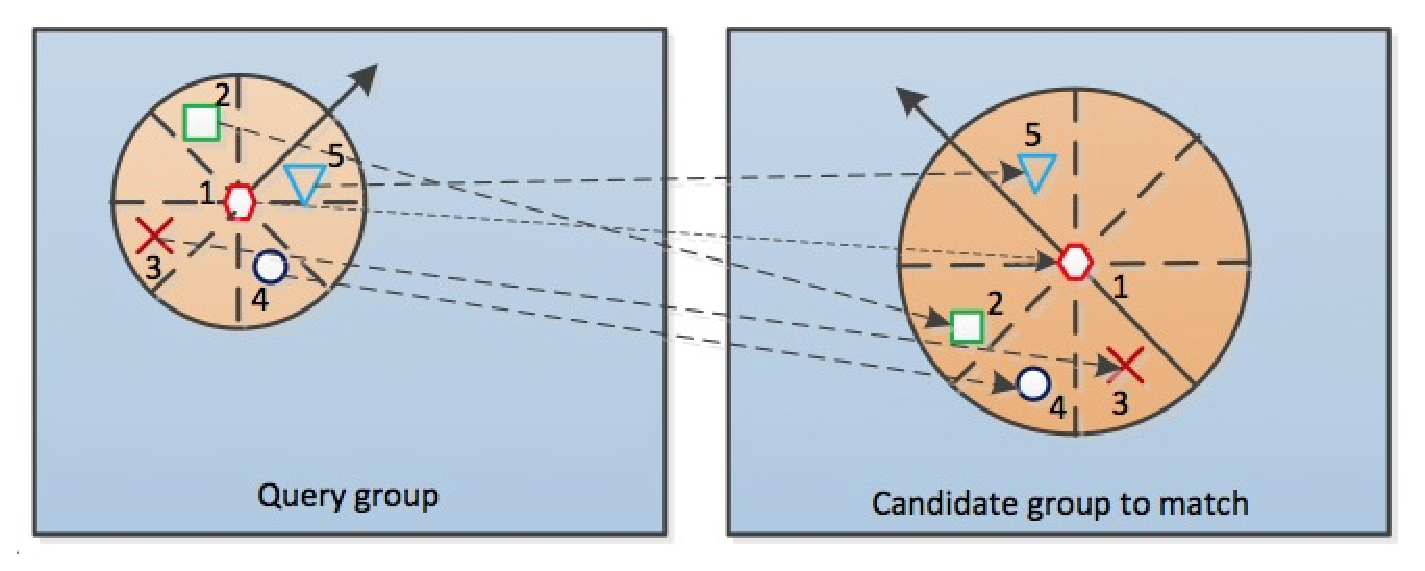
\includegraphics[width=12cm]{visual_group}
\caption{视觉词组编码方式}
\label{fig:visual}
\end{figure}


\section{系统设计}

服务器端在线重建如图\ref{fig:serverOnline}所示:
\begin{figure}
\centering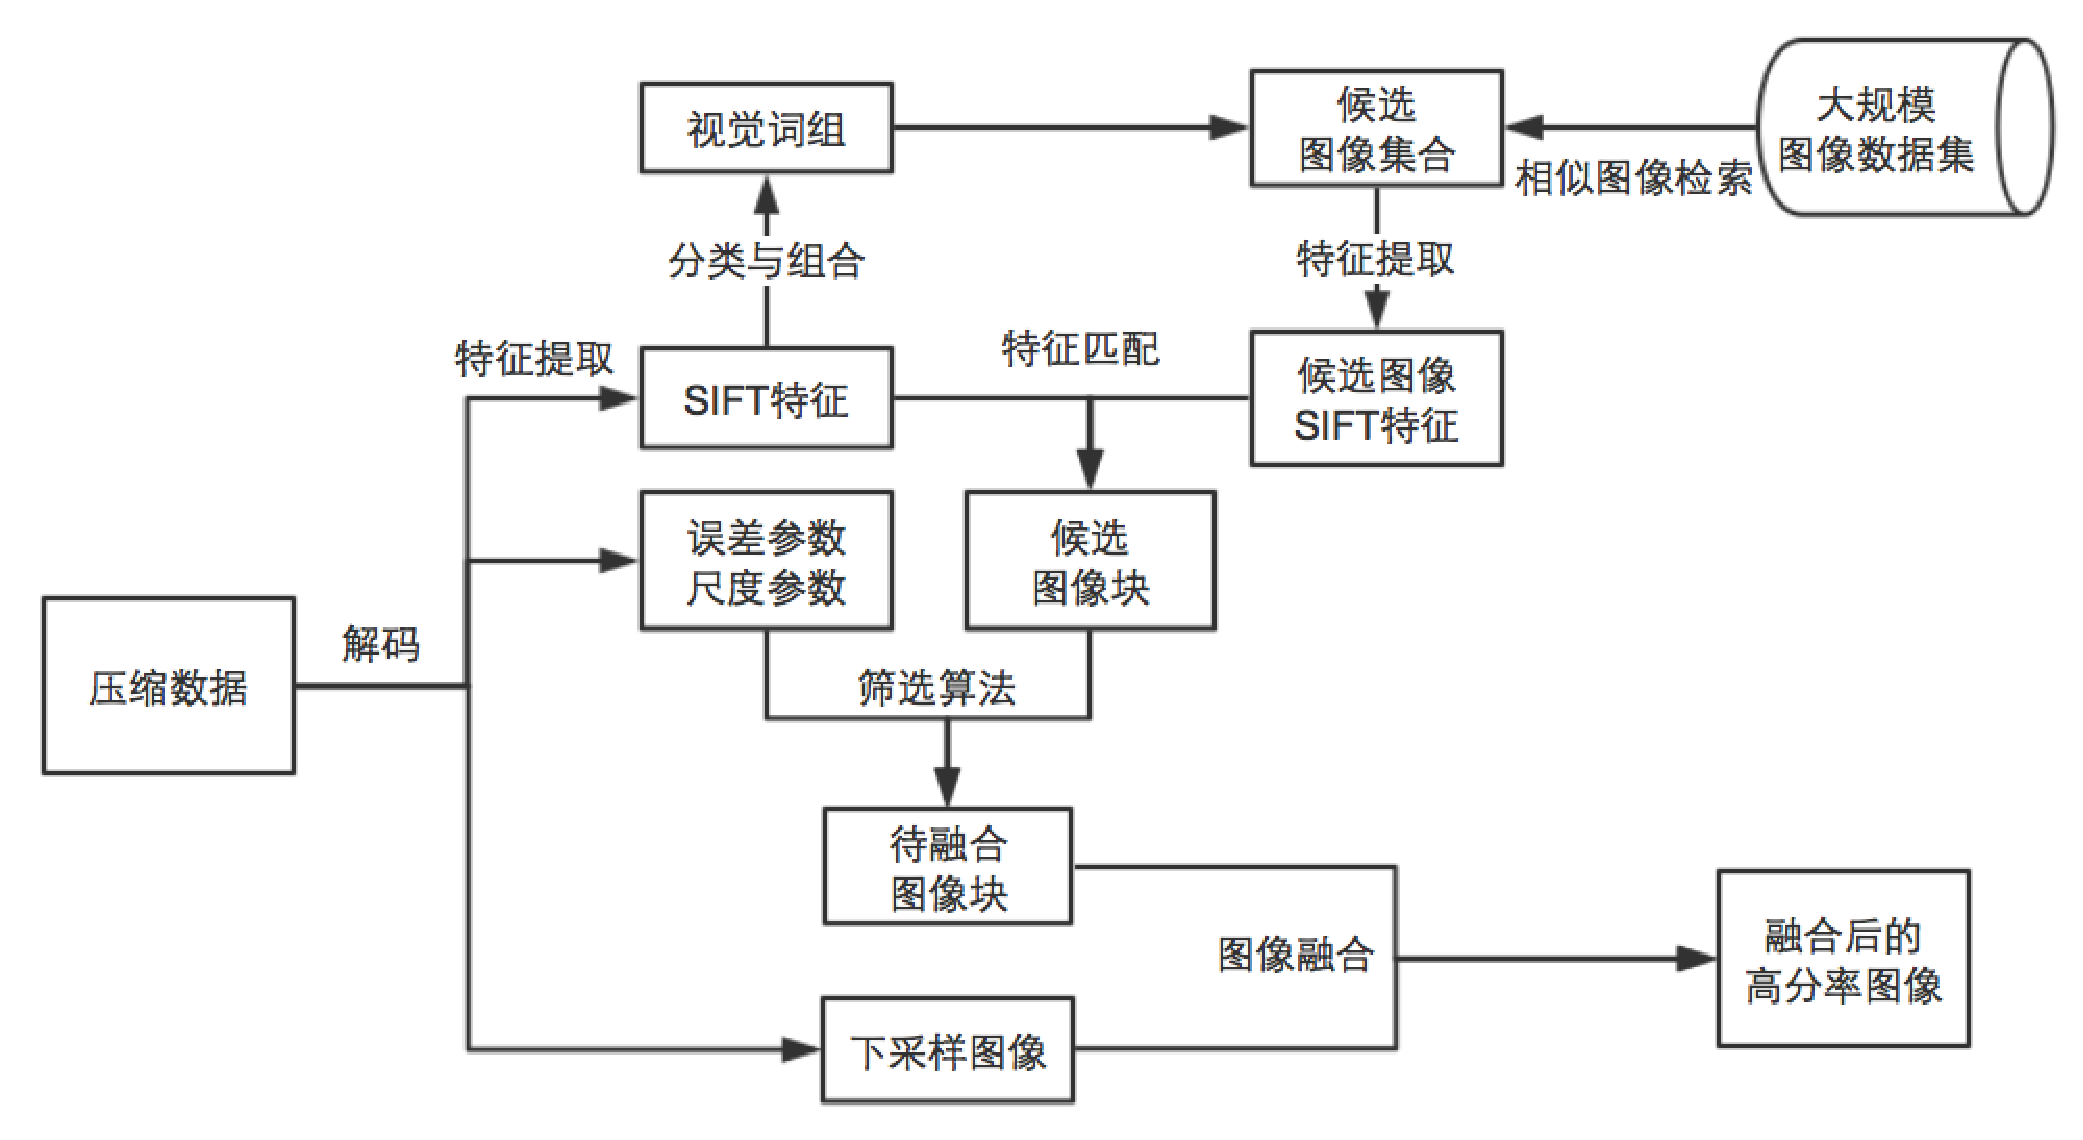
\includegraphics[width=15cm]{serverOnline}
\caption{服务器在线重建流程图}
\label{fig:serverOnline}
\end{figure}

从客户端传输来的压缩编码的数据包含了三部分信息,分别是(1)下采样图像,是1:256比例进行采样的图像,服务器端利用插值法进行上采样,恢复成原始大小得到\(I_u\);(2)SIFT关键点,传送给服务器的特征仅仅包含关键点的位置、尺度、方向等信息,不包含128维的描述子,服务器需要根据上述信息在图像\(I_u\)上重新计算特征描述,做进一步的匹配工作(3)控制信息,包括误差控制参数中的基准误差和图像块的尺度控制等,尺度控制数值与客户端提取SIFT特征计算时有关,在客户端提取时一幅图像包含各个尺度上大量的SIFT算子,通常我们需要设定一定的尺度门限,只传输门限以上的特征,这个门限可以通过SIFT算子的数量不同动态的设定。设定的门限对服务器端的候选图想块过滤起到一定的影响,所以我们将尺度门限作为控制参数传递给服务器,近一步指导候选图像块的筛选。

经过上述计算,我们解码得到三类数据,运用上文提到的视觉词组编码方式计算视觉词组,对原始图像进行分块后,在大规模图像集上利用倒排索引进行快速的相似图像搜索,得到了候选图像集合。对候选图像进行SIFT提取后与原始图像的SIFT进行匹配得到候选图像块,使用控制参数对候选图像块进行筛选得到待融合图像块,最后在下采样图像的指导下使用经典的泊松图像编辑\cite{Perez:2003ul}对图像块进行右大到小的融合,最终得到一幅高分辨率的图像。


\section{实验结果}
在实验的测试图像集中,平均每幅图像的分辨率在五百万像素以上,使用VL-FEAT图像处理函数库进行SIFT特征提取,使用其中相似K聚类(Approximately K-Means)进行视觉词的量化分类。数据集使用的是INRIA Holiday数据集\cite{INRIA},包含了500组共1491个人旅游照片。

\section{结论}

本文给出了………



%----------------------------------------------------------
% 3. 参考文献
%----------------------------------------------------------

\begin{thebibliography}{8} % 这里的2是指参考文献总数目,需要根据实际情况进行修改
    \bibitem{Dai:2012vn} Lican Dai, Huanjing Yue, Xiaoyan Sun, and Feng Wu.IMShare: instantly sharing your mobile landmark images by search-based reconstruction.pages 579--588, 2012
    \bibitem{bib2} H.E.S.Said, T.Tan and K.Baker.Personal identification based on handwriting [J].Pattern Recognition, 33:149-160, Jan. 2000
    \bibitem{bib3} 吴佑寿,丁晓青.汉字识别原理与应用[M],北京:高等教育出版社,1992.8
    \bibitem{bib4} 李航.统计学习方法[M],北京:清华大学出版社,2012.3
    \bibitem{Cloud} Huanjing Yue, Xiaoyan Sun, Jingyu Yang, and Feng Wu.Cloud-based Image Coding for Mobile Devices-Toward Thousands to One Compression, 2013.
    \bibitem{Brown:2006ir} Matthew Brown and David~G Lowe.Automatic Panoramic Image Stitching using Invariant Features.International Journal of Computer Vision, 74(1):59--73,December 2006.
    \bibitem{Perez:2003ul} Patrick P{\'e}rez, Michel Gangnet, and Andrew Blake.Poisson image editing.ACM Transactions on Graphics (TOG), 22(3):313--318, 2003.
    \bibitem{INRIA} H. Jégou and M. Douze, “INRIA Holiday Dataset,” 2008. [Online]. Available: http://lear.inrialpes.fr/people/jegou/data.php
\end{thebibliography}

\end{document}
